\documentclass[11pt]{article}



\usepackage{natbib}
\usepackage{hyperref}
\usepackage{eurosym}
\usepackage{graphicx}

\begin{document}

\setlength{\parindent}{0pt}
%first draw, fmolo, 28.10.2012
\section{economics}

\subsection{China's exports}

Exports of Chinese goods and services to the world market have risen dramatically over the last decade. %include
   
     \begin{figure}[h]
     \begin{center}
     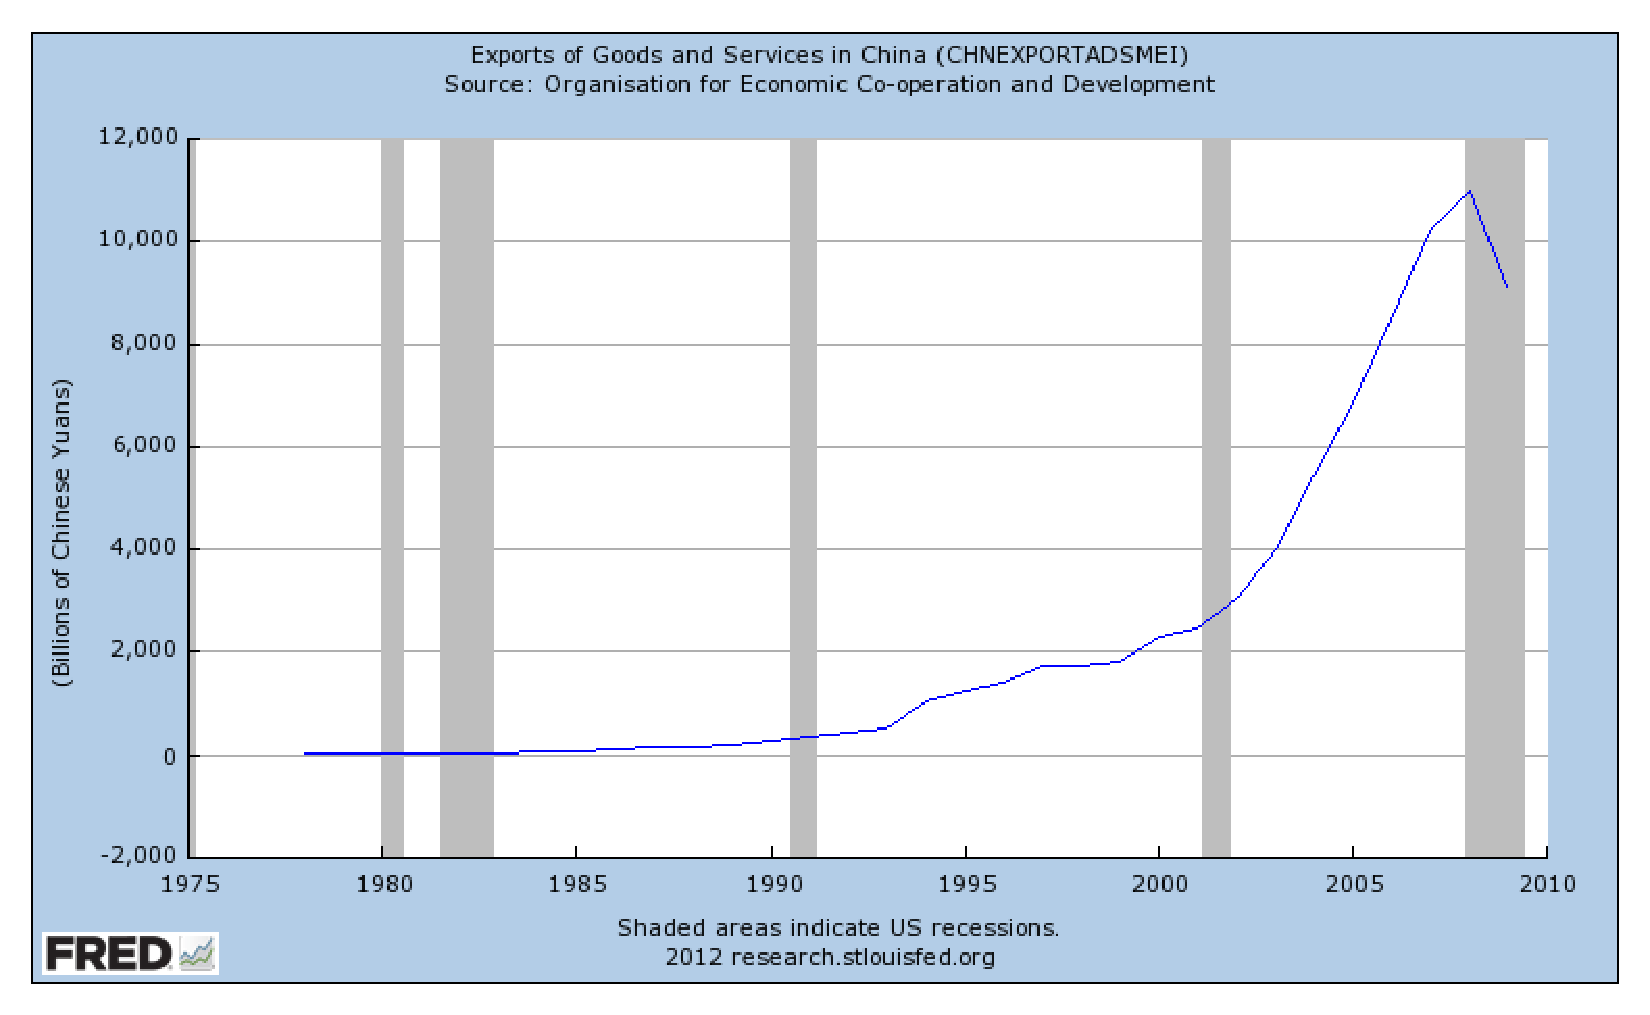
\includegraphics[width=1\textwidth]{ExportsChinaFRED.pdf}
     \end{center}
     \end{figure}

During the same period, imports of foreign goods to China have risen much less. China is taking larger share of the total world production now than it did ten years ago. Therefore, the growth of exports reflects not only the continuing integration of China's economy in the world market but also the high competitiveness of Chinese goods. 

But why are Chinese goods so competitive? First one might point out the hard work, innovation and creativity of the Chinese working force.\footnote{As \cite[p. 18]{Yu2010} indirctly does.} But economists have brought forward several other, more structural explanations.

One factor is \emph{labor arbitrage}:\footnote{This factor was hinted at by Xu Mingqi of the Institute of World economy of the Shanghai Academy of Social Sciences in a talk to our class on September 4 2012.} Chinese workers are willing to work at lower wages than workers in importing countries. Importantly, accepted wages are not only lower in absolute terms but also in terms of purchasing power: A typical wage in China allows for a lower standard of living than a typical wage in an industrial country, thereby allowing Chinese firms to produce with much lower (absolute and relative) labor costs. 

In addition to cheap labor Chinese producers find other \emph{cheap factors of production}, namely energy and land rents.\footnote{\cite[pp. 25]{Huang2010}.} These markets are not liberalized and prices can therefore be strongly influenced by government policy. Since for Chinese officials - as well on the local as on the federal level - GDP growth is a major ambition, energy and land use prices are cheaper on average than in industrial countries and even cheaper than in other emerging economies.

Another factor explaining strong Chinese exports has been introduced in 2005 by Ben Bernanke, shortly before he was named chairman of the US Federal Reserve.\footnote{\cite{Bernanke2005}}: The \emph{saving glut hypothesis}. According to Bernanke a special series of circumstances has lead to exceptionally high saving rate, i.e. the percentage of income that is saved. These circumstances include repercussions of the financial crises in emerging economies in the late 90's, but also the unique saving behaviour of Chinese households. Partly due to the lack of social security institutions and to the One-Child-Policy, the saving rate of Chinese households is among the highest in the world - in 2007 it was 53\% as opposed to Switzerland's 17,5\%.\footnote{\cite[pp. 20]{Taoyang2011}.}\footnote{Swiss Federal Statistics Office, http://www.bfs.admin.ch/bfs/portal/en/index/themen/00/09/blank/ind42.indicator.420004.420001.html.} These savings drive down interest rates in China and allow the local producers to access very cheap loans, which in turn allows them to expand production.\footnote{This explanation is also favoured by \cite[pp. 41]{Wyplosz2010}.}

Besides all these factors, \emph{China's exchange rate policy} is another factor that might possibly explain (part of) the competitiveness of Chinese goods. In order to illustrate the relevance of the exchange rate of the Chinese Currency, the renminbi (RMB), we introduce a fictional story about two companies in the next section. The story takes place in a world where we assume the RMB to be \emph{undervalued}. 





%\subsection{world market} basic idea: prices of goods. exports and imports. trade balances. current account. financial account. they depend on the following factors: x, y, z. one of these factors is the exchange rate. or: surplus would tend towards zero through the mechanism of currency appreciation (?)

% The other story:
% Let's take a look at the financial account and the current account.  
% The financial acocunt is the investments (capital) flowing in and out 
% of a country while the current account constitutes the trade balance, 
% earnings on foreign investments and cash flows (e.g. remittences).

% Per definition these two accounts balance each other in the sense that 
% if a nation has a trade deficit causing their current account to be 
% negative, the government would have to borrow money or in other words 
% let foreign governments invest in their bonds, creating a financial 
% account surplus.

% China in particular has both a trade surplus and a lot of foreign 
% investment. This leads to an advantagous situation where the National 
% Bank of China ends up with a lot of foreign currency from people 
% buying RMB to buy chinese products or construct factories in China.

% Many of the dollars that are bought by the National Bank of China are 
% reinvested into US state bonds, in effect enabling the US to keep 
% their budget deficit running.

% When the Chinese National Bank sells RMB to investors and trading 
% partners, they are in a sense free to decide how many dollars you 
% would need to buy 10 RMB. However, deciding on the exchange rate has 
% far reaching consequences that we'll get back to.

% Now, what decides the price of a product sold by a company in one 
% country to a company in another?

% 

% The third story:

% How about the following outline:
% Introduce the economy of a country like in Krugman's book as a company 
% investing money and having expenses. Explain the concepts of current 
% account and financial account in terms of these down to earth company 
% expenditures and incomes and differentiate the concepts by outlining 
% how the financial account are items that generate income while the 
% current account are items that don't.

% With this in place transplant the analogy to a country and demonstrate 
% how the different aspects map on to the economics of a country.  
% Introduce why the current account + financial account = 0 and explain 
% intuitively why that is true.

% Of course things don't work in a country like they work for a company, 
% so let's flesh out how different elements of the expenditures and 
% incomes work in a country. In particular explain how:
% - How trade between to companies in different countries work
%	[ If Migros wanted to buy Danish potatoes they would need to get 
%	hold of Danish kroners to pay the Danish farmers first. To get 
%	Danish kroners, they would buy them on the currency exchange where 
%	they would originate from Danish Banks. ...(stop here?) The Danish 
%	Banks in turn get their supply of Danish Kroners from the National 
%	Bank of Denmark. In Denmark the National Bank have decided to peg 
%	the value of the Danish Kroner to the Euro meaning that you can 
%	count on buying around 7.45dkk for 1eur. They 

% - The different shapes of foreign investment
%	[ Foreign investment comes in many shapes and forms. The most 
%	intuitive case is an example where a Swedish company invests money 
%	in a Vietnamese jungle clearing endavour in the hope of future 
%	returns. A big chunk of international investment however is done by 
%	trading state bonds. When i.e. Spain run with a budget deficit they 
%	sponsor this deficit by issuing state bonds, which basically works 
%	as I-owe-you notes with a low interest. Because states rarely fail 
%	as opposed to companies, these bonds are a very secure place in 
%	which to put your foreign currency.

%	Similarly the 


% How does the swiss national bank peg their currency at a certain rate?
 

% In order for foreign markets to buy chinese goods or invest by for 
%example constructing factories in china, they need RMB to pay with. 

% When for example the United states are drafting a new budget they 

\subsection{The story of two companies}

% TODO: Find a way to ident or otherwise mark this section to clearly 
% indicate where the story starts and ends

Based on a very successful prototype, Fluttr, a US mass manufacturer of pop art,  has decided to massproduce 
250000 miniature christmas trees made in parts with porcelain fixtures 
and in their search for a supplier they've come across MingFix, a Chinese porcelain producer,  who can 
produce fixtures at a rate much cheaper than american companies 
producing similar products. A contract is signed and Fluttr owes 
MingFix the net sum of 23 million RMB. However, Fluttr being an american 
company will have to exchange their dollars to RMB to fulfil their part 
of the contract, something they do by selling their dollars to a chinese 
bank.

% For most other currencies it's possible to easily exchange large 
% amounts of money on a currency exchange where the price of the 
% currency fluctuates with the demand and supply. However China retains 
% strict control over the access to RMB and leverages full control over 
% the value of RMB per Dollar. Currently the RMB is pegged at a fixed 
% rate to the US dollar.  This means that the exchange rate between the 
% two economies remains constant over time at 6.24RMB per Dollar. This 
% makes it easy for MingFix to sign the contract with Fluttr since none 
% of them need to worry about fluctuations in the exchange rate.  

Since the RMB is undervaluated in our hypothetic scenario both Fluttr 
and MingFix benefits from trading in RMB. For Fluttr it's advantegous 
because a good exchange rate makes the porcelain fixtures cheaper for 
them to buy, and MingFix benefits because it increases their ability to 
compete on an international market as long as they aren't reliant on 
importing products from the US.

% The dollars from the transaction ends up in the hands of the People's 
% Bank of China who aren't interested in keeping the money as is, since 
% it doesn't give them any interests and constantly loses value due to 
% american inflation. Some of the dollars are sold to Chinese buyers. 
% Some are invested in Chinese projects around the world, but a big 
% chunk of them are put in US federal bonds. These bonds are issued by 
% the US Federal Bank to cover for the trade deficit. From an american 
% viewpoint the bonds are a way to borrow money while they to the 
% Chinese is a secure way to store their american Dollars. Usually the 
% bonds will yield a bit of interest and since they are issued by a 
% nation that is very unlikely to default on its payments it is a very 
% secure way of store the dollars.

The christmas trees were a great succes and Fluttr are looking into out 
sourcing the production and decides to invest in Chinese factory 
facilities in partnership with MingFix. To start production they invest 
42 mllion RMB in China in the form of wages, land rent, buildings 
machinery and laywers typing up contracts.  This money is based on 
Dollars as before, and again the People's bank of China steps in to sell 
RMB to Fluttr for their Dollars.  Both Fluttr and MingFix benefit from a 
cheap exchange rate once again, since this gives them more value for 
their money on Chinese soil.

Half a year down the road Fluttr starts to see their market shares in 
porcelain christmas trees diminishing due to a new Chinese competitor 
calling themselves Flittle and selling similar products for much 
cheaper.  While the Dollar RMB exchange rate original benefitted Fluttr, 
they are now at a disadvantage by having large part of their design and 
administration working in the US. This makes their profit margins for 
each product sold much smaller than Flittle who benefits from a cheap 
exchange rate when they export their goods because the dollars their 
consumers pay are exchanged to RMB's at a beneficial rate.

Fluttr are forced to lay off a large part of their staff in the US as a 
response and since none of the executives are willing to relocate to 
China and start a new life there under better circumstances for their 
company, they instead spend their evenings writing angry letters to 
their senators pushing them to put pressure on China to increase the 
value of the RMB. They might have benefitted from the exchange rate for 
a while, they readily admit, but there is no way they can compete with 
an entirely Chinese company and they would much rather give up their 
collaboration with chinese suppliers than competing against chinese 
companies.

% TODO: mark the end of the story

It's important to remark in this hypothetical case that there can be 
many more reasons why a Chinese product might be cheaper than an 
American equivalent, even under the assumption that the RMB is 
undervalued. However in the counter scenario where the Chinese RMB is 
not undervaluated, several things change. Fluttr might be less reluctant 
to enter the Chinese market given that they have less purchasing power 
per Dollar. It might well be that an alternative American supplier of 
porcelain fixtures can provide competing prices. This difference is even 
more pronounced when it comes to investing in Chinese production 
facilities. Both the initial investment as well as the goods produced by 
the facilities become more expensive as the RMB increases in value in 
relation to the American Dollar.

\subsection{A bit of analysis}

The above example shows in a simplistic way how the exchange rate that 
People's Bank of China charges for changing Dollars into RMB could have 
an impact on american and chinese companies. Both the size and fairness 
of this impact are however heavily disputed on a diplomatic level 
between China and the US as well as in academic circles.

To understand these arguments, it's necessary to introduce a few 
fundamental concepts. We base these concepts on introductory texts in 
economics that are generally agreed upon in the field of economics.  
However as will become obvious once we explore the arguments on either 
side of the debate, even fairly fundamental issues can sometimes be 
interpreted in more than one way. We will try as best we are able to 
illustrate these ambiguities in an impartial fashion.


% However what it doesn't show is the flip side of a cheap Dollar/RMB 
% exchange rate to the Chinese consumer. For an ordinary Chinese factory 
% worker, having a cheap RMB might in on sense mean that their factory 
% is doing great on foreign markets, but at the same time buying foreign 
% products like european cars or american gadgets becomes near 
% impossible. 

\subsection{foreign exchange market}

Money is a tradable good and different currencies can be traded against 
each other in the foreign exchange market. Market participants such as 
private persons, corporations, commercial banks and national banks can 
exchange a certain amount of a currency for another amount of another 
currency. This exchange takes place either at commercial banks and 
currency exchanges on an open market as with the Dollar, or by trading 
with state owned banks under tighter restrictions as with the RMB. The 
exchange rate as introduced in the story of Fluttr and MingFix is the
price of a currency A in terms of currency B. On an open market, the 
exchange rate is determined by supply and demand for a currency. If at 
some point the demand for more US dollar rises, for example because a 
international corporation invests in the US and pays workers there a 
wage in US dollars, the price of the dollar on the currency market will 
be higher, i.e. you will get fewer US dollars for one euro. However 
nations can chose to exercise a tighter control of the value of their 
currency by different measures.

On of the means nations have to control the value of their currency is 
their national bank. In principle, each national bank has an unlimited 
supply of its own currency, because they can - figuratively speaking - 
print a discretionary amount of money in their own 
currency.\footnote{The process is somewhat more complicated than 
printing bank notes, but the effect is the same for the purposes of this 
section.} A national bank can therefore influence the exchange rate of 
its currency against other currencies. If the national bank of the US, 
the US Federal Reserve decides to print more US Dollars and uses them to 
buy euros, the price of the dollar in terms of euro depreciates, i.e.  
you will get more US dollars for one euro.

\subsection{The tempting misuses of a national Bank}

In our story about MingFix and Fluttr we show how manipulating an 
exchange rate can be beneficial for a nation focused on export and 
foreign investments. However this behaviour forces trading competitors 
to take similar steps in order to protect their own exports, which 
easily leads to a situation where countries are competing to devaluating 
their currencies in order to compete. Historically this behaviour was 
recognized as nonbeneficial for all partners involved and international 
institutions was instantiated to create a set of rules for all partners 
involved. The most prominent of these today are the IMF (International 
Monetary Fond), the WTO (World Trade Organization) and the EU (European 
Union).

However deciding exactly when the rules are broken and a country is 
gaining an unfair advantage can be difficult in practice. China has been 
accused by prominent US politicians of `manipulating' its currency and 
keeping the Chinese currency, the Renminbi\footnote{abbreviated to CNY. 
The basic unit of the Renminbi is the Yuan.} `undervalued'. The next 
section will analyze how this alleged manipulation takes place and what 
it means for a currency to be undervalued.


% I've taken this out since I think we should introduce it later when we 
% talk about china pegging the yuan to the dollar

% This process is very common: Some national banks even use their money 
% supply to `peg' their currency to another, so that exchange rates are 
% fixed.  For example, the Swiss National Bank (SNB) offers every vendor 
% of an euro CHF 1.20 in exchange.  Since the SNB controls the money 
% supply of Switzerland, it will never run out of CHF and the exchange 
% rate of the Swiss franc. As a consequence the euro will never be lower 
% than 1.20 until the SNB changes its exchange rate policy.  As another 
% example, the national bank of Denmark controls the supply of Danish 
% kronor so that the exchange rate of the kronor and the euro constantly 
% remains at 0.134 (with a small bandwith of +/-2.25\%).

% Such practices seem to be accepted in public discourse and by the 
% relevant multilateral agency, the International Monetary Fund.  
% Meanwhile, China has been accused by prominent US politicians of 
% `manipulating' its currency and keeping the Chinese currency, the 
% Renminbi\footnote{abbreviated to CNY. The basic unit of the Renminbi 
% is the Yuan.} `undervalued'. The next section will analyze how this 
% alleged manipulation takes place and what it means for a currency to 
% be undervalued. 

\subsection{nominal undervaluation, currency manipulation}

Macroeconomic theory postulates, that for every two currencies at every 
moment, there is an equilibrium exchange rate. The equilibrium exchange 
rate is determined by supply and demand for each currency in the foreign 
exchange market. The accusation against China of `manipulating' its 
currency can therefore be restated: It claims that China is keeping a 
fixed exchange rate \emph{below} the equilibrium rate. According to 
textbook economics this can be done in three ways:\footnote{\cite[pp. 
514]{Krugman2008}}

\begin{enumerate}
\item{The government can shift supply and demand for its currency by intervening on the foreign exchange market. Buying foreign exchange and selling the local currency drives the price of foreign exchange up and that of the local currency down.}
\item{The government can shift supply and demand by means of monetary policy, namely by keeping interest rates low. Lower interest rates mean lower returns for foreign investors. If foreign investors refrain from investing locally, the demand for the local currency decreases, driving the price of the local currency down.}
\item{The government can impose foreign exchange controls, forbidding foreigners to buy the local currency, therefore again reducing demand and therefore the price of that currency.}
\end{enumerate}

Yet each of these practices have legitimate purposes making it difficult 
to argue that the mere use of these techniques necessarily indicates a 
manipulative monetary policy. For example Switzerland has since the 
onset of the great recession applied the first technique to 'peg' the 
swiss franc to the euro. In essence the Swiss National Bank (SNB) offers 
every vendor CHF 1.20 in exchange for an euro. Since the SNB controls 
the money supply of Switzerland, it will never run out of CHF and the 
exchange rate of the Swiss franc. As a consequence the euro will never 
be lower than 1.20 until the SNB changes its exchange rate policy.  As 
another example, the national bank of Denmark controls the supply of 
Danish kroner so that the exchange rate of the kronor and the euro 
constantly remains at 0.134 (with a small bandwith of +/-2.25\%).  
Neither of these techniques have provoked action from any of the 
international bodies governing currency manipulation.


% Why would a government do such things? Goods produced in a country 
% with a low exchange rate are cheap relative to goods produced in other 
% countries, since production costs are paid in the (low-valued) local 
% currency. A low exchange rate therefore increases competitiveness of 
% the export sector. 

\subsection{China criticism}

Without being able to pinpoint illegal measures, how can we argue that a 
currency is indeed undervalued? The logical approach to answer this 
question would seem to be a comparison between the equilibrium exchange 
rate and the current exchange rate. However while attempted, this method 
proves difficult to the point where many economists argue that there is 
no reliable method to determine the `right' exchange rate of a 
currency.\footnote{among others: \cite{pp.  4}{GoldsteinLardy2008}}
%Purchasing power parity (PPP) would possibly be a method, but I have not seen it discussed in relation with China yet.

Critics of China therefore base their case on circumstantial evidence 
rather than on hard empirical methods using one of two methods. Either 
they can correlate the equilibrium exchange rate with other economic 
factors and approximate it by looking at these factors. Alternatively 
they can look at the actions of the Chinese government and argue that 
China's economic policy couldn't have any other valid purposes than to 
keep its currency undervalued.

\subsubsection{Estimating the equilibrium exchange rate}

There exists various different theoretical methods for estimating an 
equilibrium exchange rate in the litterature. However, to understand 
them it's necessary to introduce the notion net foreign asset (NFA) as 
well as the concepts of current and foreign account (CA and 
FA)\footnote{For a more in depth explanation \cite{ch.  
18}{KrugmanTextbook} provides a good introduction}.

The net foreign asset is the value of the assets that a country owns 
minus the value of assets from that country which is owned abroad.  
Assets in this sense is usually state bonds but can also be stocks and 
goods.  

The current and financial account are measures for how the NFA changes.  
The current account constitutes the balance of trade and money transfers 
while the financial account constitutes the balance of financial assets, 
that is the debt or amount of money lent to other countries. 

The two accounts are related by the current account plus the financial 
accout being equal to zero. This makes sense intuitively since if a 
nation buys more goods than it can finance with exports it needs to 
finance this by selling state bonds instead. In this case, the negative 
trade balance translates to a current account deficit, while the influx 
of money coming from the sale of state bonds translates to a finance 
account surplus.

When it comes to estimating the equilibrium exchange rate these three 
measures are heavily used because they gives us an idea of how stable an 
economy is, judging from how assets and goods are flowing in and out of 
the economy. In particular a report was released in 2008 by the 
Internation Monetary Fund outlining three methods that can be used to 
estimate the disparity between the real and equilibrated exchange 
rate\footnote{The Report: \cite{pp.  1}{Lee08}}:

\begin{enumerate}
\item{The macroeconomic balance approach looks at projections of a 
	country's current account and tries to estimate how much the 
exchange rate would need to be adjusted for it to stabilize within a 
certain level}
\item{The reduced-form equilibrium real exchange rate approach tries to 
	estimate the equilibrium directly as a function of the NFA as well 
as a number of trade indicators}
\item{The external sustainability approach tries to find the exchange 
	rate that would stabilize the NFA of a country to within a certain 
level}
\end{enumerate}

In practice these techniques has been used by Cline and Williamson in 
their yearly policy brief on equilibrium exchange 
rates\footnote{\cite{cline2009,cline2012}}.  Their estimates are based 
largely on the first and third methods proposed by the IMF, designating 
debt and trade surplus above 3\% of GDP as abnormal and calculating how 
much the exchange rate would have to change to bring the current account 
within a normal treshold. In 2009 their results showed that the Chinese 
RMB was undervaluated by 21.4\%, a number which has been much quoted 
since then. Especially in relation to the fact that they found the US 
dollar 17.4\% percent overvaluated, futher contrasting the value gab 
between the two currencies.

Instead of trying to find the equilibrium exchange rate, a different 
approach is to do the exact opposite. If we pick a comparative point in 
time or statistical measures based on other countries, we can measure 
how much the current exchange rate deviates from a factor that remains 
constant.

If we pick the unit price of labour as our constant and 1998 as our 
point of reference it is straightforward to show that the RMB is 25 
percent undervalued when compared to at least the American 
Dollar\footnote{\cite{chimerica2009}}. Similarly we can focus on the 
purchasing power parity (PPP)\footnote{The PPP is a measure for how the 
price for similar goods and services in two countries differ}. Based on 
the behaviour of poor countries in growth based on the PPP, it is 
estimated that the RMB is undervalued between 12\% and 
47\%\footnote{\cite{Subramanian2010}}.

% It's really funny that this text (Subramanian2010) is quoting Cline 
% and Williamson as well as Goldstein and Lardy for agreeing on the same 
% number, when in fact Goldstein and Lardy have their number from Cline 
% and Williamson (2009)

% Also from the same paper:
% Since each of the four estimates suffers from limitations, a 
% reasonable approach would be to average all four. This yields an 
% undervaluation estimate for China of about 31\% against the dollar, 
% which is my preferred PPP-based estimate.
% who are giving grants to these people?

\subsubsection{The alleged purpose of China's economic policy}

The argument against how China conducts its economic policy compared to 
the measures a country would take to undervaluate their currency is 
stated by Goldstein and Lardy\footnote{\cite[pp.  
40]{GoldsteinLardy2008}} as follows:

\begin{enumerate}
\item{The Chinese government has intervened on the foreign currency 
		market on a massive scale: It has been buying foreign 
		currencies, mainly US Dollars (in the form of US government 
		debt) in exchange for RMB to the amount of 10\% of its GDP, i.e. 
		10\% of the value of all goods and services produced in China.} 
		%show data. but first find data (IMF? FRED?)
\item{Interest rates in China are relatively low, with real (i.e. adjusted for inflation) interest rates actually being negative for the most part since 2006.} %show data. but first find data (World Bank?)
\item{China imposes foreign exchange controls that prevent international investors or other governments to buy RMB.}%this seems clear, but i have not yet found how they do it exactly
\end{enumerate}

As a result, critics of Chinas exchange rate regime say, China's export sector has become extremely competitive. Indeed, China's exports exceed its imports by far; in absolute terms, such a current account surplus (i.e. the amount by which the value of exports exceed the value of imports) is unprecedented, though not so much in relative terms. %account surplus data is easily available. including switzerland might be fun, because the Swiss surplus is even higher. 

%is monetary policy used for normal goals (like controlling inflation) or is it used to manipulate the currency? for some countries these goals align (switzerland), but not so for china (inflation is high, and they still sell RMB)
 
\subsection{nominal vs. real exchange rates}

If the Chinese government chooses option (1) above and buys foreign currency paying with RMB, it is increasing the amount of money in the economy.\footnote{In economical jargon it is expanding the \emph{monetary base}, what (other things equal) leads to an increase in money supply} According to standard economic models\footnote{\cite[pp. ?]{Krugman2008}} an increase in the money supply raises the price level in the domestic economy, leading to inflation.\footnote{Maybe quickly explain the assumed mechanism?} As a result, goods produced in China would become more expensive on the world market not due to currency appreciation, but because production costs (e.g. wages of Chinese workers) rise with inflation. According to this model, even though the People's Bank of China (PBC) keeps the \emph{nominal} exchange rate fixed, the \emph{real} exchange rate, i.e. the exchange rate would float.\footnote{\cite[p. 509]{Krugman}} Therefore, inflation would in the long run offset the competitive advantage of Chinese goods on the world market gained by the low(er) nominal value of the RMB.

China has indeed seen some inflation during the last ten years. But so did other countries - the real and the nominal exchange rate roughly moved in unison during the last ten years.\footnote{source: http://www.clevelandfed.org/research/trends/2010/1110/01intmar.cfm}%find data to display
Critics of China attribute this to China's \emph{sterilization} of the money inflows. Since 2003, China hast prevented about 40\% of the money inflows of entering the monetary base by raising reserve requirements of Chinese commercial banks.\footnote{IMF, via Cleveland Fed, http://www.clevelandfed.org/research/trends/2010/1110/01intmar.cfm}%display data?
Raising reserve requirements limits the amount of loans the commercial banks can issue, therefore 'extracting' money out of the economy. This in turn limits inflation and prevents the real value of the RMB to rise. This is another manifestation of China manipulating the RMB exchange rate: Not only does it keep the nominal exchange rate artificially low, it also intervenes on the real exchange rate, preventing the 'natural' offset on nominal currency manipulation.



\subsection{China apology}


\subsection{newest developments; the situation by now (2012)}


\end{document}
